%% This is an example first chapter.  You should put chapter/appendix that you
%% write into a separate file, and add a line \include{yourfilename} to
%% main.tex, where `yourfilename.tex' is the name of the chapter/appendix file.
%% You can process specific files by typing their names in at the 
%% \files=
%% prompt when you run the file main.tex through LaTeX.
%% prompt when you run the file main.tex through LaTeX.
\chapter{Use of a Global Model to Understand Atmospheric Mercury Observations at Monitoring Sites in Latin America }
%% BACKGROUND
\begin{flushleft}
Environmental pollution from Hg can damage ecosystems through its transformation into toxic methylmercury and bio-accumulation in food chains. Further, Hg is highly mobile in the atmosphere, allowing it to travel to faraway places, resulting in worldwide distribution of its elemental form, \hg, which can last for as long as six months in the atmosphere\cite{horowitz_new_2017,shah_improved_2021}. Hg in the atmosphere can be classified as gaseous elemental Hg (GEM), gaseous oxidized Hg (GOM), and particulate-bound Hg (PBM) less than 2.5$\mu$m in diameter \cite{lindberg_synthesis_2007,schroeder_atmospheric_1998,landis_development_2002}. In most cases, Hg emissions occur as gaseous elemental Hg0, which is relatively inert and sparingly soluble in water\cite{horowitz_new_2017}. Since most Hg entering ecosystems comes from the atmosphere, monitoring and modeling atmospheric Hg and Hg deposition enables us to understand its biogeochemical cycle. In addition, a better understanding of Hg's circulation in the environment would enable effective policies to reduce its harmful effects.
\end{flushleft}
\section{Background}
\begin{flushleft}

Hg monitoring networks and atmospheric Hg models are closely interconnected in the literature. For instance, Gustin et al., (2015) analyzed the state of the science of monitoring and modeling Hg in the atmosphere to deal with the challenge of developing links between Hg ambient levels, deposition, and ecosystem contamination. Notably, the mutual dependency between atmospheric modeling and monitoring is presented in the MC's "Guidance on Monitoring Mercury and Mercury Compounds to Support the Effectiveness Evaluation of the Minamata Convention," which states that observations are needed not only to detect and quantify changes, but also to improve and evaluate models of mercury transport, fate, exposure, and impacts\cite{unep_guidance_2021}. Similarly, Sprovieri et al. emphasize the importance of making consistent global Hg measurements to validate regional and global-scale models\cite{sprovieri_atmospheric_2016}.  According to Brasseur and Jacob, (2017), it is crucial to have a large ensemble of observations to evaluate atmospheric Hg modeling outputs, and several studies have published results using different ensembles of Hg monitoring data. For instance, Weiss-Penzias et al,(2015) used the GEOs-Chem model to develop an understanding of speciated atmospheric mercury observations at five high elevation sites(4 in the USA and 1 in Taiwan)\cite{weiss-penzias_use_2015}. Until now, no detailed model comparison has been conducted in some world regions with high anthropogenic Hg emissions, such as Latin America. The lack of high-frequency atmospheric Hg monitoring capacity in these regions may have limited studies comparing observations to models in these regions, as shown in Figure \ref{fig:global-hg-monitoring-networks}, which illustrates the distribution of global Hg monitoring networks published in the GMA 2018. As seen in Figure \ref{fig:global-hg-monitoring-networks}, Latin America, Africa, and South East Asia remain significantly behind Europe and North America regarding access to relevant observation ensembles. 
\end{flushleft}

\begin{figure}[H]
  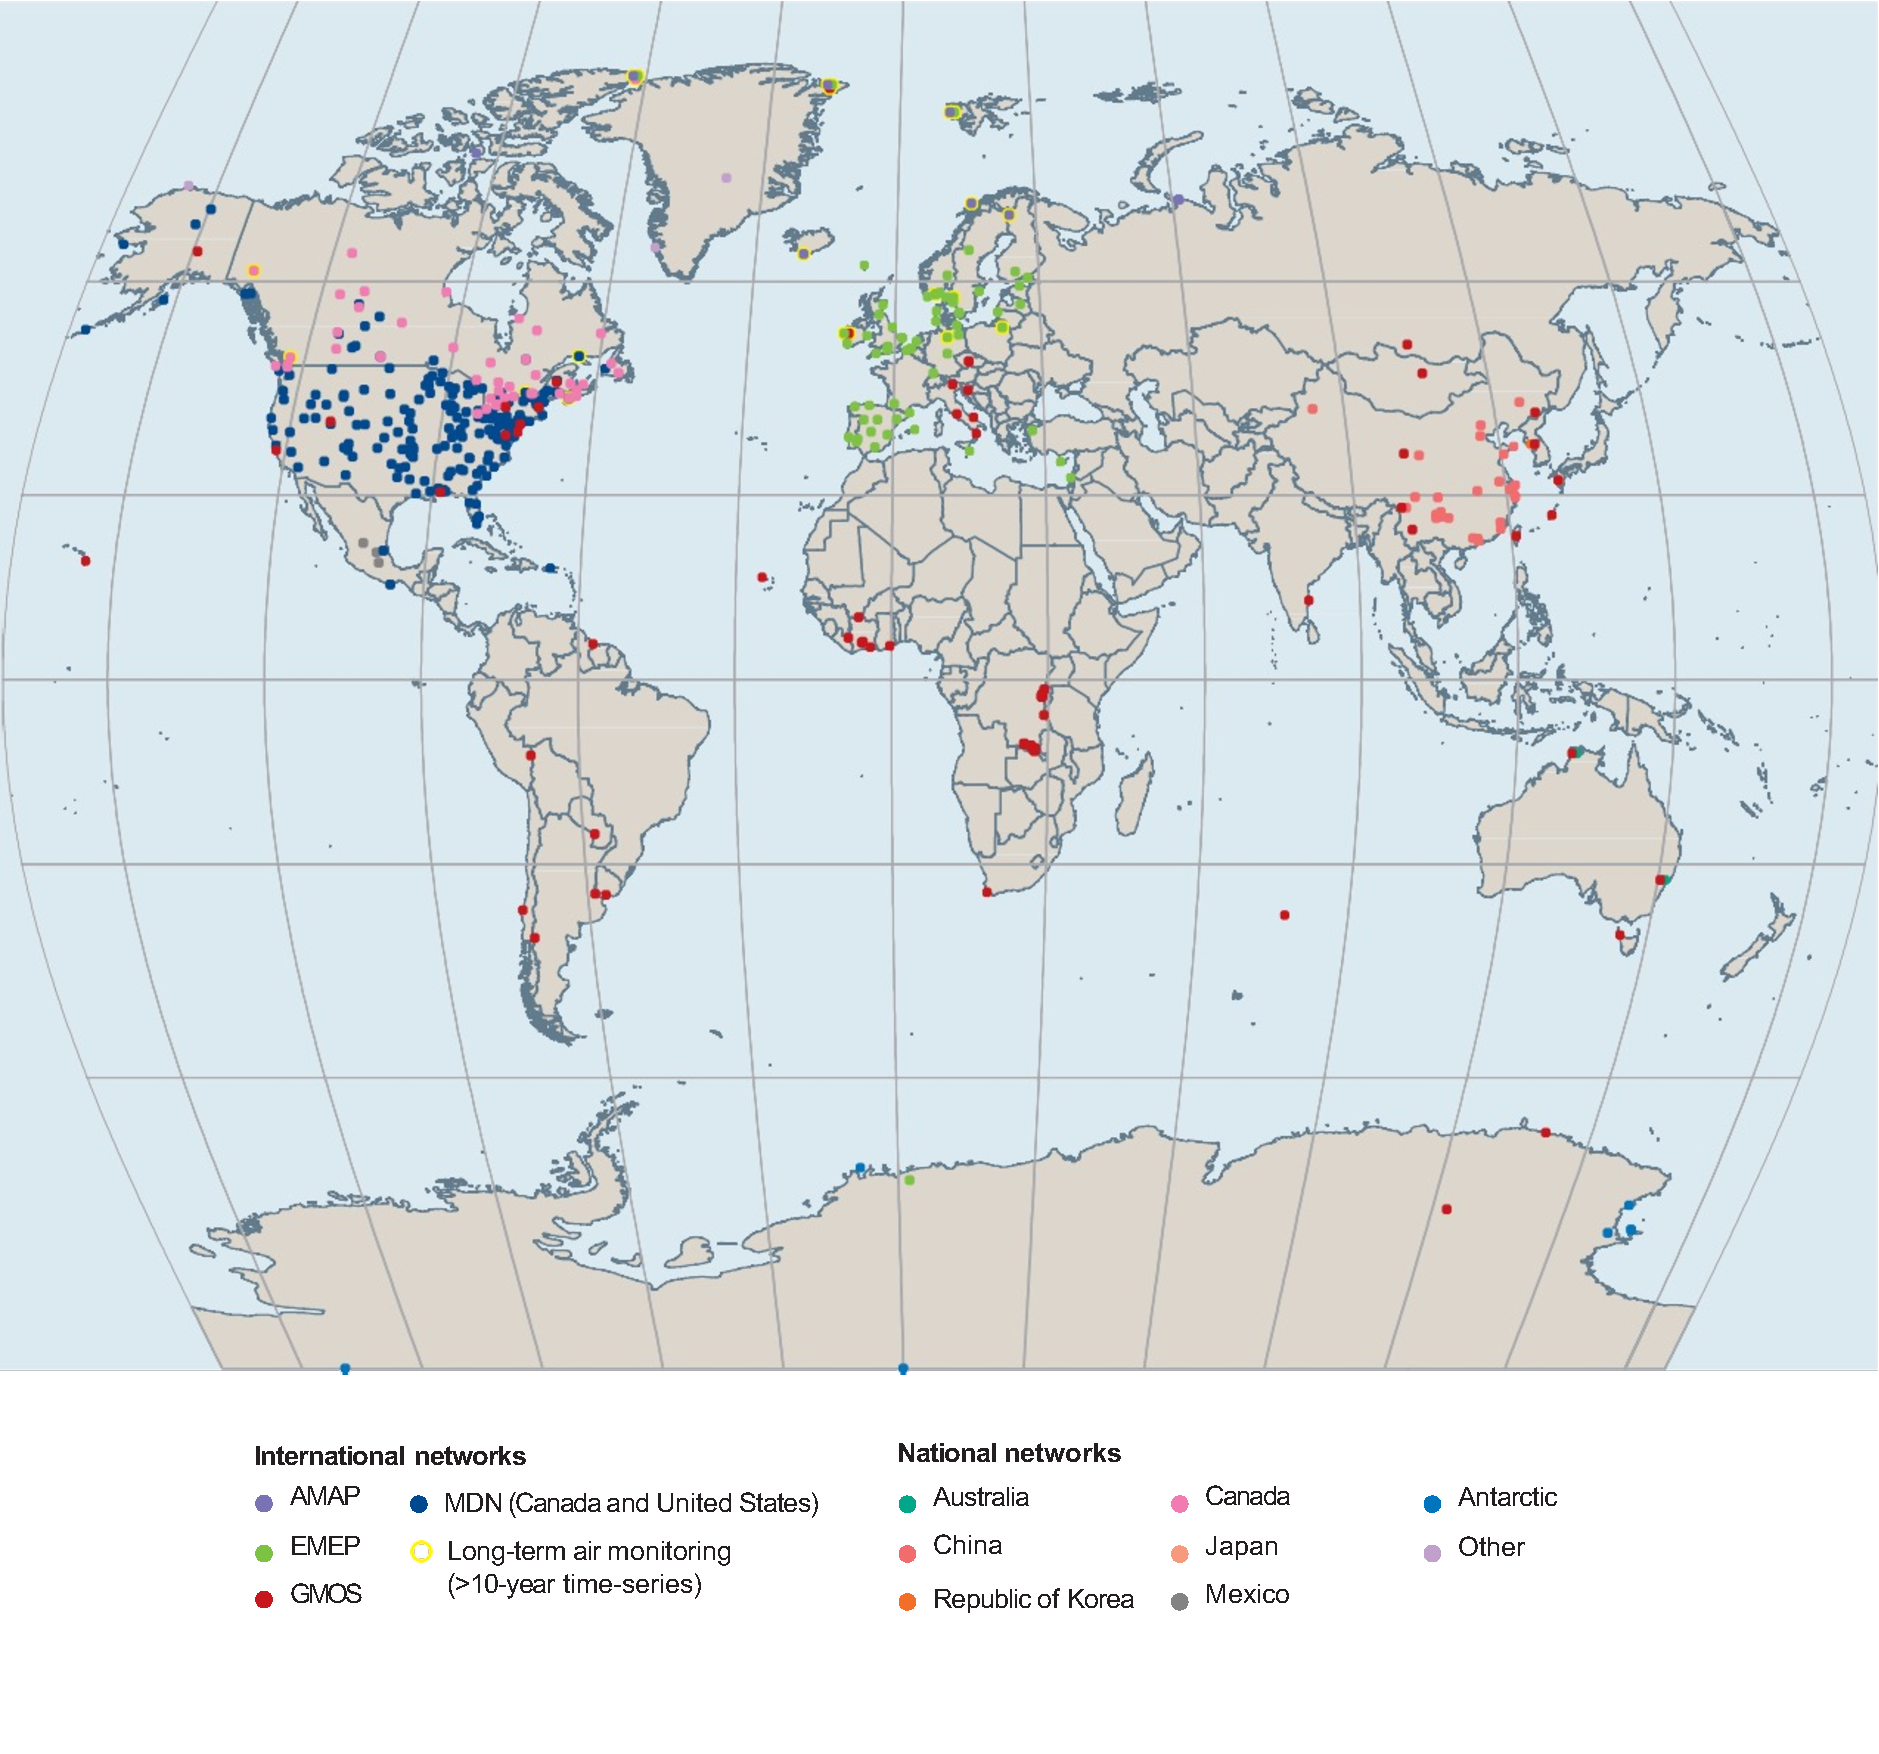
\includegraphics[width=\textwidth]{templates/figures/global-hg-monitoring-networks.pdf}
  \caption{Global map of Hg monitoring networks \cite{united_nations_environment_programme_technical_2019}}
  \label{fig:global-hg-monitoring-networks}
  \centering
  
\end{figure}
\FloatBarrier

\begin{flushleft}
 In this chapter, I compare outputs of the GEOS-Chem model with observed Hg at multiple sites in Latin America. I combine simulations of Hg in the atmosphere produced by the \gc CTM (Sect. 2.2.1) with ground-based observations of atmospheric total gaseous mercury (TGM) (Sect. 2.2.2) from the Global Mercury Observation System (GMOS)\cite{sprovieri_atmospheric_2016} and gaseous elemental mercury (GEM) data from a network of passive air samplers (PAS) distributed across Latin America. Section 2.3 presents results and discussion\cite{quant_measuring_2021}. Comparisons of observations and model outputs are given in Sect. 2.3.1. Finally, I discuss the implications of the current state of atmospheric monitoring and modeling atmospheric Hg in Latin America (Sect. 2.3.2) and summarize my conclusions (Sect. 2.4).
\end{flushleft}




%%----------------------------METHODS-------------------------------------------
\section{Methods}
\subsection{GEOS-Chem Description}
\begin{flushleft}


The global atmospheric Hg concentration was simulated using version 12.8.1 of GEOS-Chem, whose Hg simulation is described by Horowitz et al. (2017)\cite{horowitz_new_2017}. All the simulations in this study were run globally for 47 vertical layers at a resolution of 2.0$\times$2.5, which is approximately equal to a 222 km$\times$277.5 km grid square at the equator \cite{horowitz_new_2017}. Moreover, the MERRA-2 assimilated meteorological data,\cite{gelaro_modern-era_2017} drive the model's atmospheric transport, which calculates atmospheric Hg from three tracers: elemental Hg, Hg\textsuperscript{0}, divalent Hg, Hg\textsuperscript{2+}, and particulate-bound divalent Hg,Hg\textsuperscript{p}. The Hg chemical scheme in the GEOS-Chem version used in this study considers bromine (Br) to be the primary \hg oxidant\cite{horowitz_new_2017} and employs monthly mean Br oxidant concentrations from Schmidt et al.,(2016)\cite{schmidt_modeling_2016}. 
\end{flushleft}
\begin{flushleft}
\subsection{GEOS-Chem Simulations}
The GMA 2018 emissions inventory was used to represent anthropogenic emissions sources from all sectors\cite{steenhuisen_development_2019}. Different inputs to the GEOS-Chem model, such as emissions sources, can be toggled on or off depending on the research objective; hence a reference simulation, \on was created by turning on all Hg emissions sources globally. Moreover, a \off was generated by turning off the ASGM source globally to evaluate the contribution of ASGM to the baseline \hg in the atmosphere by calculating the difference between the \on and \off.
\end{flushleft}


\begin{table}[H]
\captionof{table}{Description of GEOS-Chem Simulations Conducted}
\label{tab:geos_chem_simulation_description}

\centering
\resizebox{\textwidth}{!}{\begin{tabular}{lcp{0.6\linewidth}}

Simulation Name  & Resolution & Description  \\
                        
\hline
Base (ASGM=ON)         & 2.0$\times$2.5 & All Hg anthropogenic emission sources are turned on  \\
No ASGM (ASGM=OFF)        & 2.0$\times$2.5 & All ASGM emissions are turned off

\end{tabular}}

\end{table}
\begin{flushleft}
 The frequency of the simulation output was set to output daily \hg averages at the global scale, while the \hg output for the grid boxes corresponding to the locations of the GMOS observation sites was set to an hourly frequency. The GEOS-Chem outputs for all the simulations conducted were in units of parts per trillion (ppt) and were converted to \nang at standard temperature and pressure (273 K, 1 atm) to compare them to observations.
\end{flushleft}

\subsection{Monitoring Site Characteristics}
\begin{flushleft}
 The GMOS network is one of a few major global projects to develop a global observing system for mercury pollution. GMOS aims to provide high-quality Hg data sets in the Northern and Southern hemispheres to enable a more comprehensive assessment of atmospheric Hg concentrations and their dependence on meteorology, long-range atmospheric transport, and atmospheric emissions\cite{sprovieri_atmospheric_2016}. A vast network of ground-based monitoring stations, regular oceanographic cruises, and lower, upper, and stratospheric measurements make up this European Union-funded project \cite{koenig_seasonal_2021,sprovieri_atmospheric_2016}. More than 40 ground-based monitoring sites constitute the international network, covering many regions with limited to no observational data available before GMOS\cite{sprovieri_atmospheric_2016}. The GMOS monitoring network has five sites in Latin America that actively monitor Hg levels. An analysis of the characteristics of the Sisal, Calhau, Manaus, Nieuw Nickerie, and Bariloche sites has been published by Sproviery et al., (2016), and the Chalcataya site has been analyzed in detail by Koenig et al., (2021) \cite{koenig_seasonal_2021,sprovieri_atmospheric_2016}. A summary of the sites' characteristics is shown in Table \ref{tab:gmos_sites_info}  and they are shown by red triangles in Figure \ref{fig:Latam_Passive_SamplerSites}. A primary objective of this study was to evaluate the degree to which ASGM Hg emissions affected the Hg concentrations in the atmosphere at regional and global scales, so high-frequency GMOS data were collected to facilitate this evaluation.
  \end{flushleft}
  
  \begin{table}[H]
\captionof{table}{The GMOS Sites Evaluated \cite{koenig_seasonal_2021,sprovieri_atmospheric_2016}. }
\label{tab:gmos_sites_info}

\centering
\resizebox{\textwidth}{!}{\begin{tabular}{llccp{0.2\linewidth}rcll}
  \hline

Site                        & Site      & Latitude  & Longitude & Physical  & Elevation    & Number of      & Site &  Measurement  \\
                            & abbrev    &           &           &  Setting  & (m)           & Records (days) & Type&   Period \\
\hline
Sisal, Mexico               & SIS       & 21.16     & -90.05    &   Coastal site        &   7           &   320 &   Secondary    & 1/1/2010-1/1/2016   \\
Calhau, Cape Verde          & CAL       & 16.86     & -24.87    &   Coastal site        &   10          &   309 &   Secondary   & 1/1/2013-12/1/2014  \\
Nieuw Nickerie, Suriname    & NIK       & 5.93      & -56.98    &   Coastal site        &   1           &   215 &    Secondary   & 3/1/2007-12/1/2014 \\
Manaus, Brazil              & MAN       & -2.89     & -59.96    &    Amazon site       &  110          &   100 &   Master   & 1/1/2013-12/1/2014 \\
Chalcataya, Bolivia         & CHC       & -16.2     & -68.12    &    Mountain site       &  5340         &   333 &    Secondary   & 7/1/2014-2/1/2016  \\
Bariloche, Agentina         & BAR       & -41.13    & -72.42    &    Mountain site       &  800          &   333 &  Master     & 10/1/2012-7/1/2017 \\
  \hline
\end{tabular}}

\end{table}

  
 \begin{flushleft}
  The GMOS sites are classified as either secondary or master sites in Table\ref{tab:gmos_sites_info} to indicate the type of data collected and the type of equipment used at the site. The secondary sites used the Tekran continuous mercury vapor analyzer, model 2537A/B (Tekran Instruments Corp., Toronto, Ontario, Canada), except for the Nieuw Nickerie site (NIK), Suriname, which used a Lumex RA-915+ mercury analyzer. The master sites used the Tekran model 2537A/B mercury vapor analyzer coupled with their speciation system model 1130 for GOM and model 1135 for particulate boundaries mercury (PBM2.5) with fractions less than 2.5 $\mu$m in diameter to prevent large particles from depositing on the KCl-coated denuder \cite{koenig_seasonal_2021,sprovieri_atmospheric_2016,gustin_measuring_2015}
     
 
\end{flushleft}

\begin{figure}[H]
 \centering
  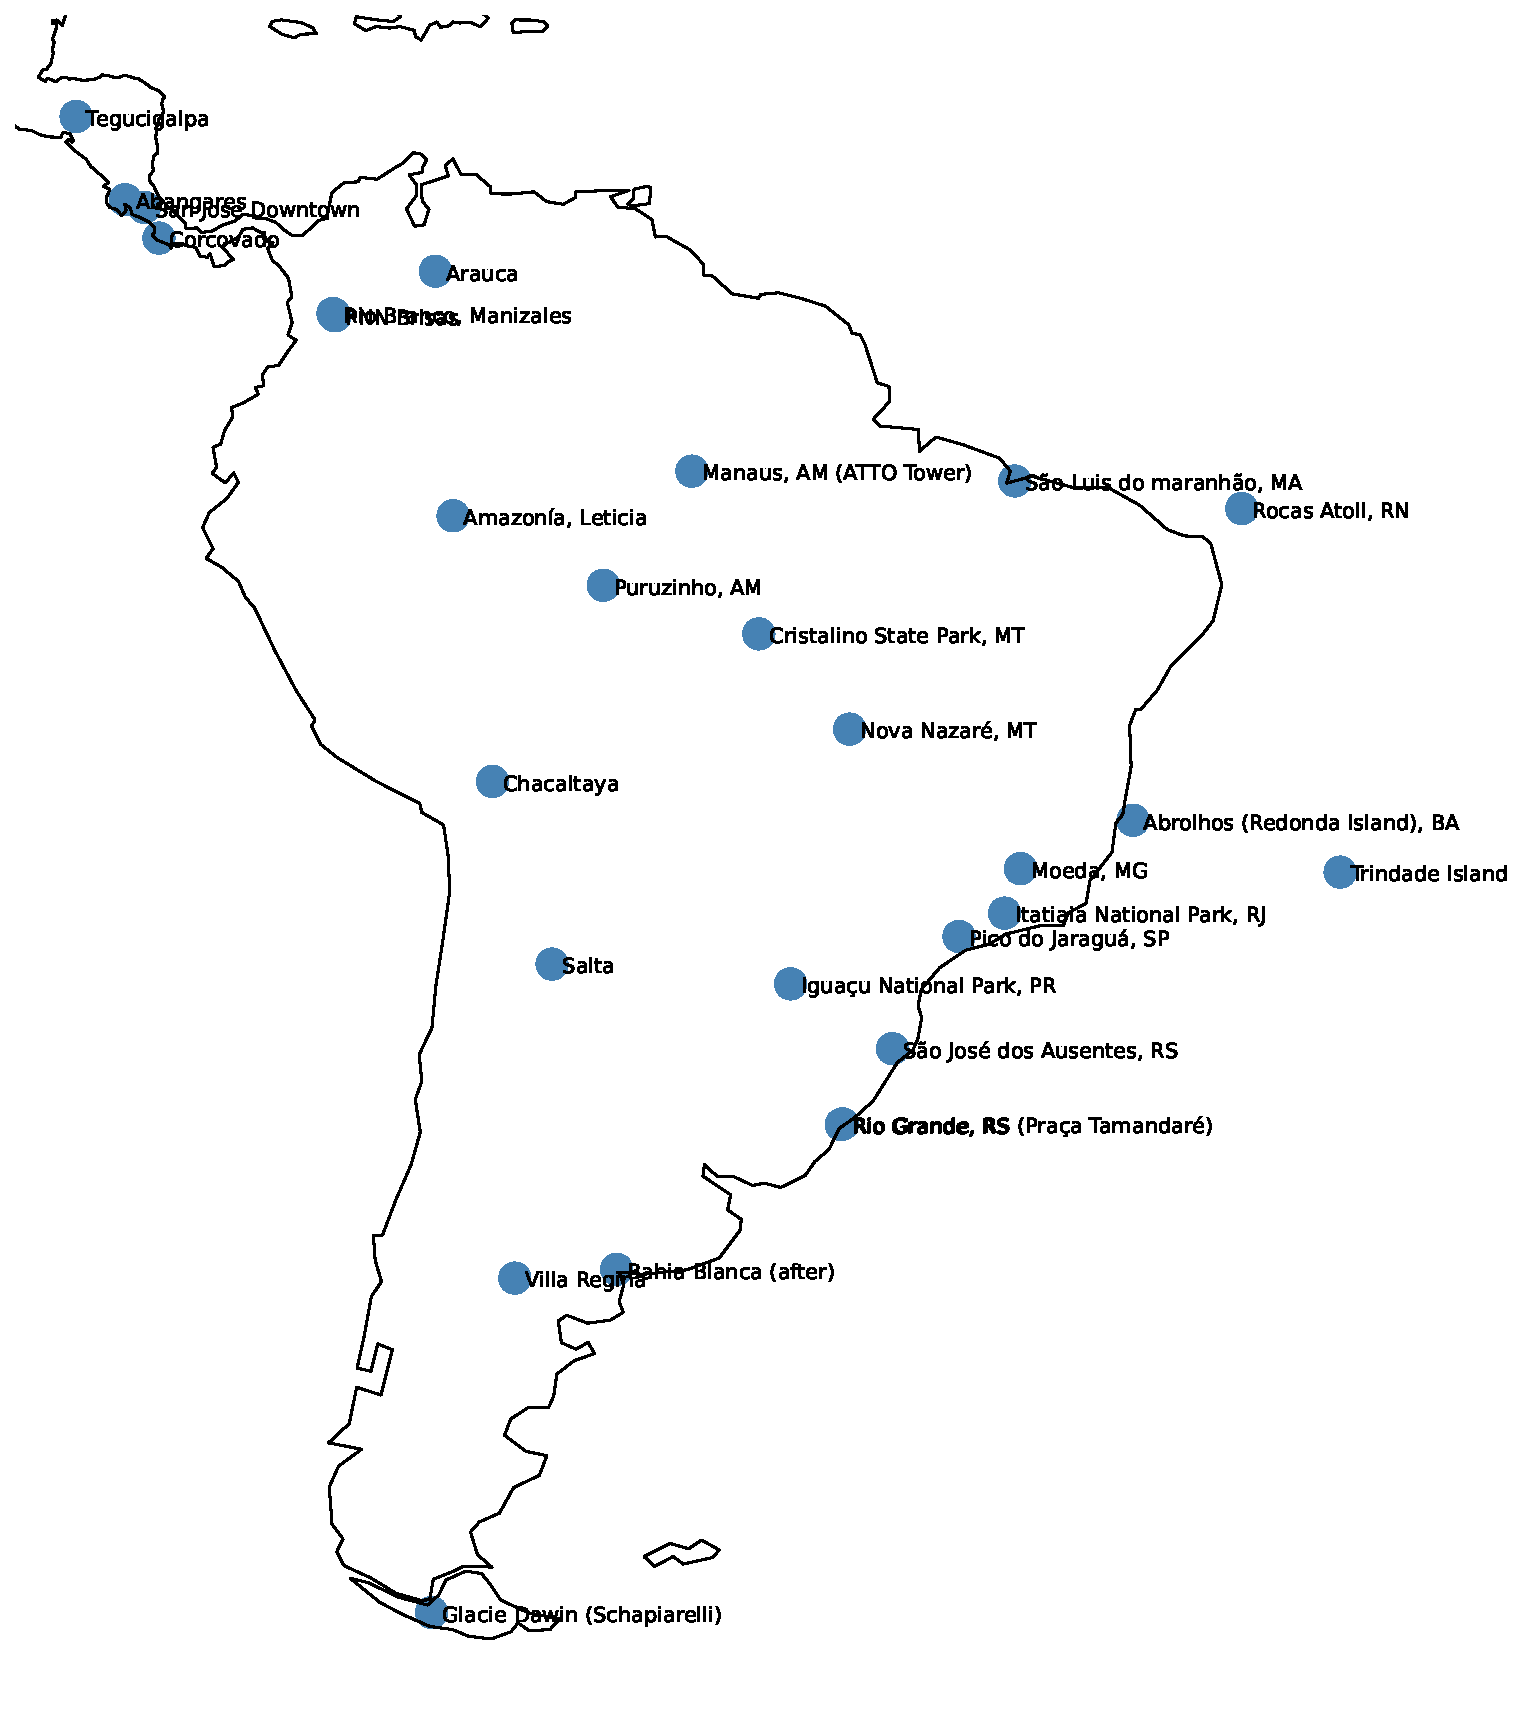
\includegraphics[width=0.8\textwidth]{templates/figures/Passive_Samplers/Latam_Passive_SamplerSites.pdf}
  \caption{Map Showing the GMOS Monitoring Network Sites and Passive Sampler Locations in South America \cite{quant_measuring_2021,koenig_seasonal_2021}}
  \label{fig:Latam_Passive_SamplerSites}
\end{figure}
\FloatBarrier

\begin{flushleft}
    In contrast to active Hg monitoring equipment such as those used in the GMOS network, which can be prohibitively expensive, energy-intensive, and require extensive training, passive air samplers (PAS) require no energy to operate and do not require any special handling skills \cite{quant_measuring_2021}. Furthermore, PAS can be easily deployed for long periods. This combination of attributes of PAS allows more sampling sites to be studied over extended periods enabling significant average GEM concentration estimates to be obtained. PAS monitoring is integral in informing the effectiveness evaluation of the MC\cite{gustin_measuring_2015,unep_guidance_2021}. Quant et al.,(2021) published a detailed analysis of the PAS sites in Latin America, and their respective locations are shown by the blue circles in Figure \ref{fig:Latam_Passive_SamplerSites}. 
\end{flushleft}

\subsection{Observation Data Sourcing Manipulation}
\begin{flushleft}
  Additionally, average annual GEM concentration data for 27 sites in Latin America was obtained from Quant et al.,(2021), which included information about the coordinates of the deployment sites and the period of measurement \cite{quant_measuring_2021}. Available Hg observation data from the GMOS stations on Figure  \ref{fig:Latam_Passive_SamplerSites} was obtained from the GMOS online database (http://www.gmos.eu), as well as published studies about the Hg monitoring data from the different sites  \cite{koenig_seasonal_2021}. The data sets were pre-processed based on the information in Sproviery et al.,(2016) and Koenig et al.,(2021) and daily and annual averages to compare with the \gc output\cite{koenig_seasonal_2021,sprovieri_atmospheric_2016}. The PAS data was compared to the modeled annual average Hg concentration for 2015 to evaluate, and the coordinate information from the PAS data was used to directly compare the GEM observations and model outputs at the respective PAS sites.
\end{flushleft}





%%----------------------------RESULTS AND DISCUSSION---------------------------
\section{Results and Discussion}

\begin{figure}[H]
\centering
  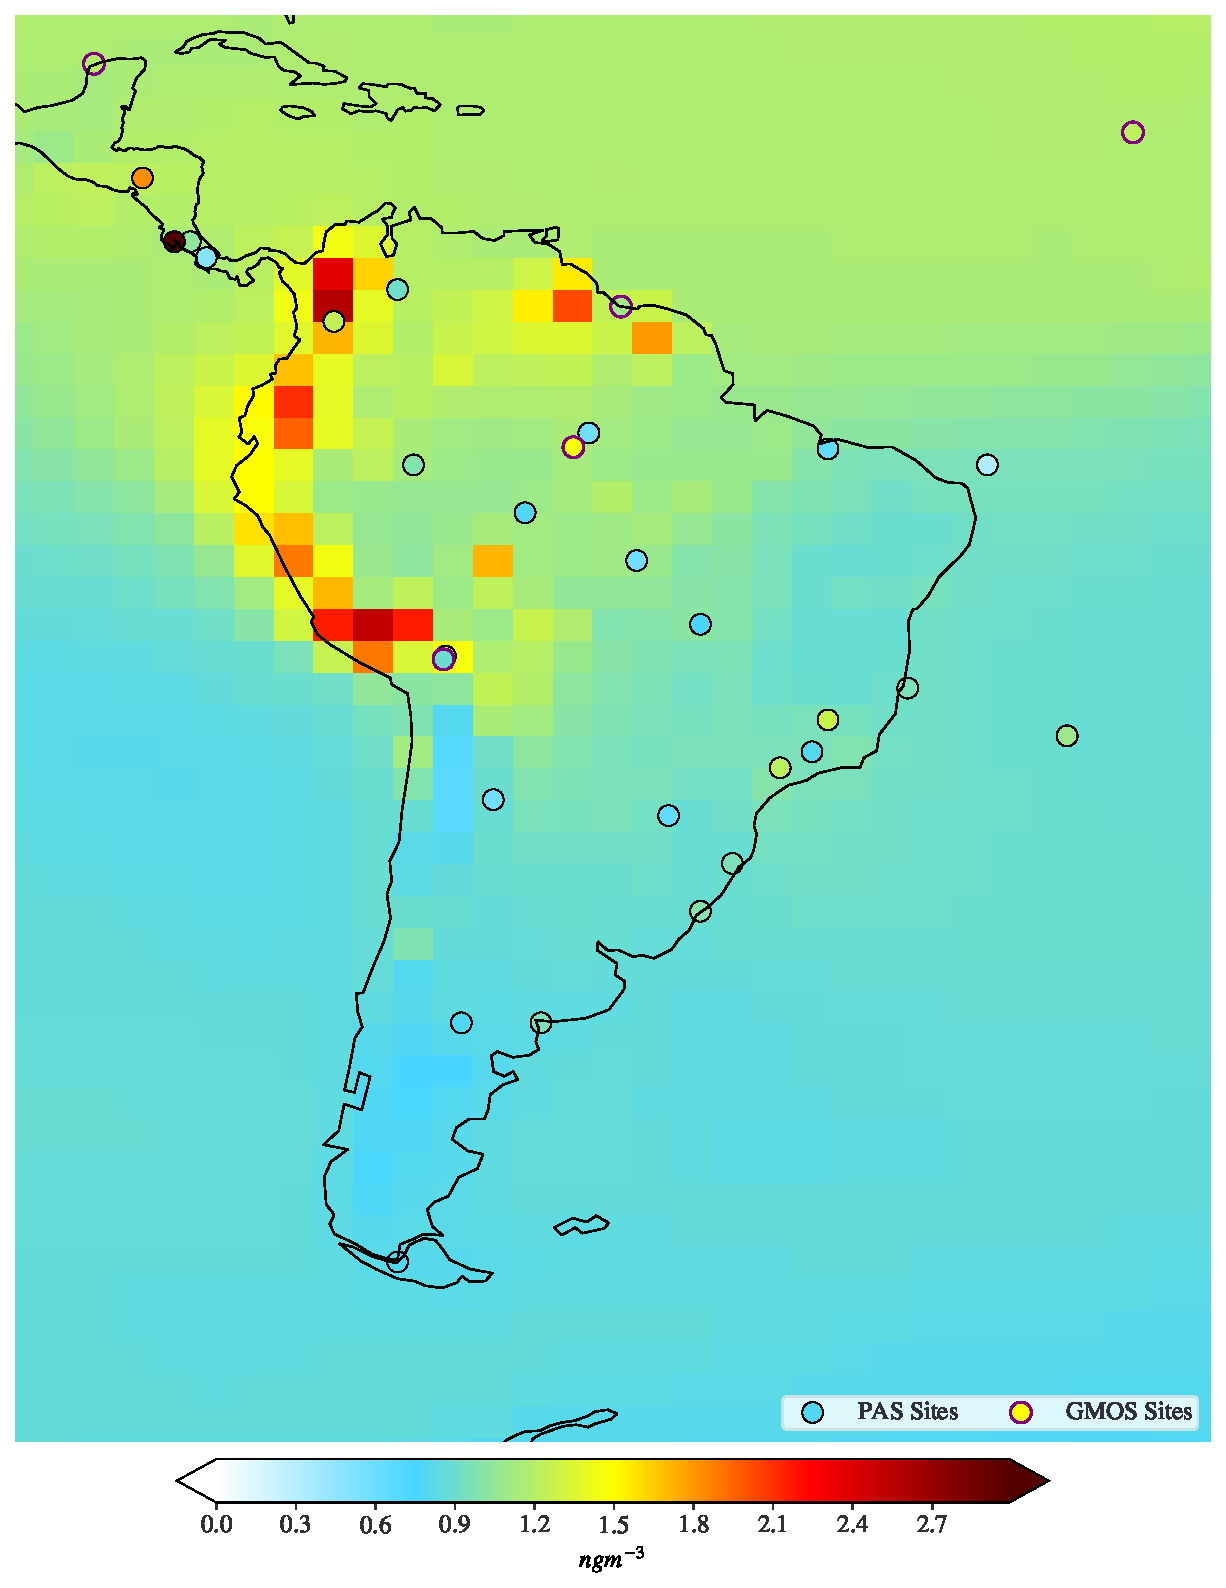
\includegraphics[width=0.7\textwidth]{templates/figures/Passive_Samplers/07-27-22_pas_vs_model_Hg0-per-year_001.pdf}
  \caption{Annual average Hg concentration on the surface in Latin America averaged. The background is the annual average \hgc produced by the \on for 2015. The circles are the annual average GEM concentration from the PAS sites, while the triangles are the annual average TGM concentrations from the GMOS sites.\cite{quant_measuring_2021,sprovieri_atmospheric_2016,koenig_seasonal_2021}}
  \label{fig:06-12-22_pas_vs_model_Hg0-per-year_001}
  
  
\end{figure}
\FloatBarrier
\begin{flushleft}
 Recent publications analyzing global Hg monitoring data highlight an observed interhemispheric gradient of Hg where Hg concentration in the southern hemisphere is lower than Hg concentration in the northern hemisphere\cite{sprovieri_atmospheric_2016}. This gradient is evident in the simulated background annual average \hg concentration as seen in Figure \ref{fig:06-12-22_pas_vs_model_Hg0-per-year_001}. Moreover, most of the GMOS sites validate the modeled interhemispheric gradient except the Chalcataya GMOS site. The model matches the PAS GEM measurement at Chalcataya. This may be explained by the fact that the GMOS Chalcataya Site is a high-altitude site where the Hg concentration was measured at 5340 m above sea level, yet the modeled background shown in Figure \ref{fig:06-12-22_pas_vs_model_Hg0-per-year_001} is the Hg annual average on the surface. Compared with PAS data, the GEOS-Chem model overestimates atmospheric concentrations. Inland sites exhibit this phenomenon more than those located along the coast. There is a difference between the model and the inland PAS sites, especially those in the Amazon region because this version of the GEOS Chem model underestimates Hg uptake by vegetation. Figure \ref{fig:06-12-22_pas_vs_model_Hg0-per-year_by-latitude_001} which shows the modeled (blue circles) and observed (red circles) annual average \hg plotted as a function of latitude clearly indicates the interhemispheric gradient observed in GEOS-Chem. The observation error bars represent the replicate precision of the observations, while the model error bars represent the 95\textsuperscript{th} bootstrap confidence interval for the mean annual \hg. As opposed to the GMOS sites, where GEOS-Chem overestimates the concentrations at all sites, GEOS-Chem only overestimates the concentrations at 15 of the PAS sites, and four of these sites are within the error bars. Evident on Figure \ref{fig:06-12-22_pas_vs_model_Hg0-per-year_by-latitude_001}  is that \gc underestimates Hg concentrations at low latitudes and overestimates those at high latitudes. However, this trend is addressed by the vegetation uptake argument since the Amazon forest is in the northern latitude of Latin America.
\end{flushleft}

\begin{figure}[H]
  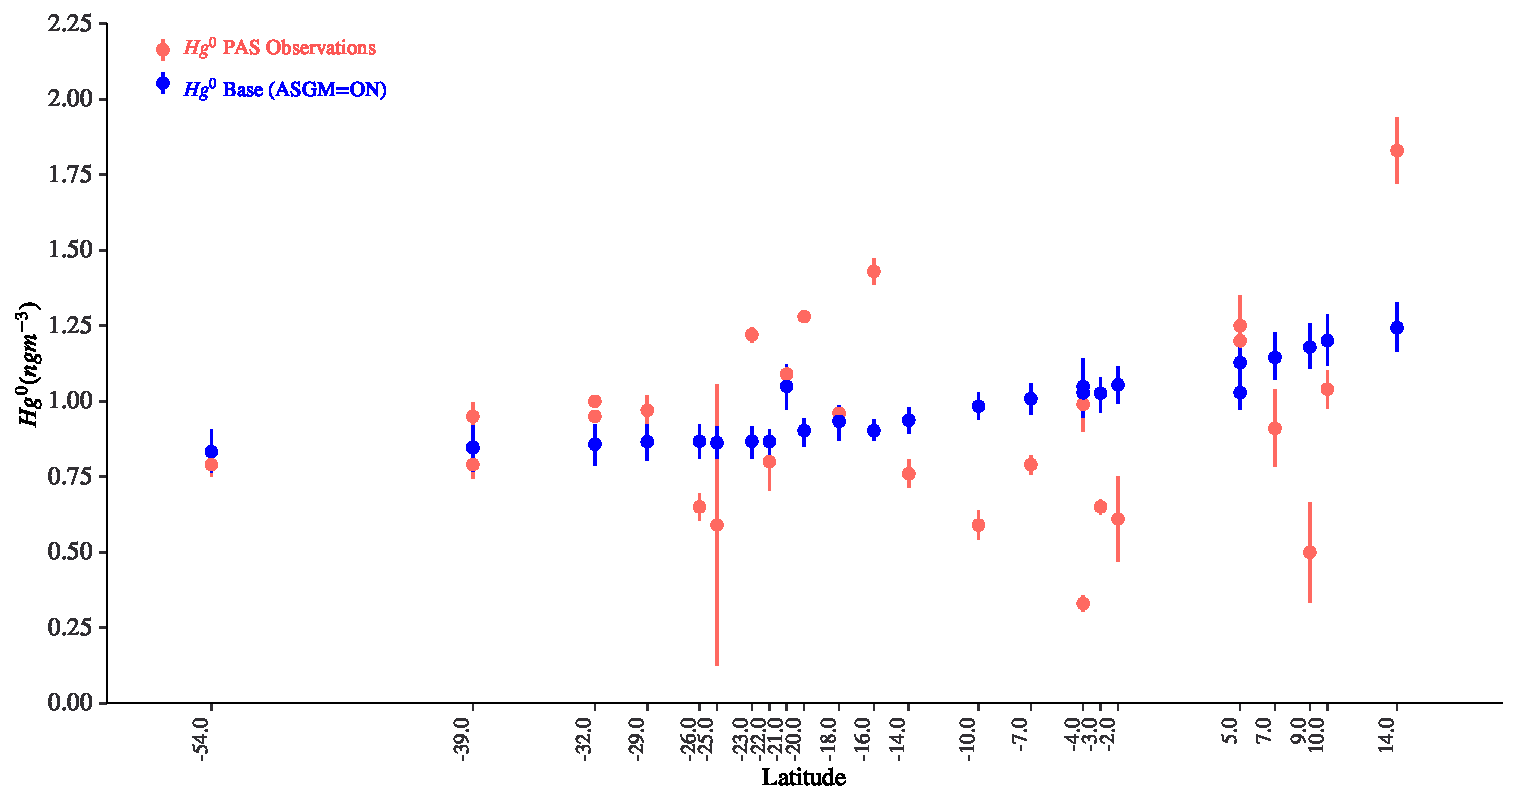
\includegraphics[width=\textwidth]{templates/figures/Passive_Samplers/06-12-22_pas_vs_model_Hg0-per-year_by-latitude_001.pdf}
  \caption{\hg in the atmosphere as a function of Latitude. The \on (blue circles) and observed (red circles) annual average \hg plotted are plotted as a function of latitude to evaluate spatial trends across the continent. The observation error bars represent the replicate precision of the observations while the model error bars represent the 95\textsuperscript{th} bootstrap confidence interval for the mean annual \hg.}
  \label{fig:06-12-22_pas_vs_model_Hg0-per-year_by-latitude_001}
  \centering
  
\end{figure}
\FloatBarrier
\begin{flushleft}
    \gcs overestimation of Hg concentration in the Amazon region observed above was also addressed in Feinberg et al. (2022), who compared simulations with litterfall, throughfall, and flux tower measurements from 93 forested sites to evaluate vegetation as a Hg sink. According to their results, the \gc version, 12.8 underestimates \hg dry deposition, which may explain why measurements of Hg concentration in Latin America were lower than predicted by \gc. 
    
    % Furthermore, the PAS measurements, as seen in Figure \ref{fig:06-12-22_pas_vs_model_Hg0-per-year_001} were higher in most of the eastern coastal regions and in the northwestern coastal regions. These high values result from the PASs being placed near populated areas where the Hg background in the atmosphere may also be influenced by Hg emission sources such as power generation and ASGM. At the Amazon sites, however, low GEM measurements highlight the importance of vegetation as a Hg sink. 
\end{flushleft}
% \begin{table}[H]
% \captionof{table}{The comparison of the model predictions of the average Hg concentration for the available measurement period}
% \label{tab:ASGM_at_GMOS_annual_avs}

% \centering
% \resizebox{\textwidth}{!}{\begin{tabular}{lcccccc}
%   \hline

% GMOS & Observed Hg\textsuperscript{0} & Observation Standard & Base(ASGM=ON) Hg\textsuperscript{0} & Base(ASGM=ON) Standard  & ASGM Contribution  Hg\textsuperscript{0}   \\
% Sit & (ng m$^{-3}$)/year             & Deviation ($\sigma$) & (ng m$^{-3}$)/year                   & Deviation ($\sigma$)      &(ng m$^{-3}$)/year\\
                        
% \hline
% Sisal           &   1.19    & 0.14 & 1.27 & 0.05 & 0.12  \\
% Calhau          &   1.22    & 0.12 & 1.30 & 0.04 & 0.11  \\
% Niew Nickerie   &   1.11    & 0.23 & 1.41 & 0.06 & 0.25  \\
% Manaus          &   1.49    & 0.31 & 1.27 & 0.09 & 0.23  \\
% Chalcataya      &   0.90    & 0.16 & 1.20 & 0.14 & 0.28  \\
%   \hline
% \end{tabular}}

% \end{table}
\subsection{Modeled vs Observed Temporal Trends}
\begin{figure}[H]
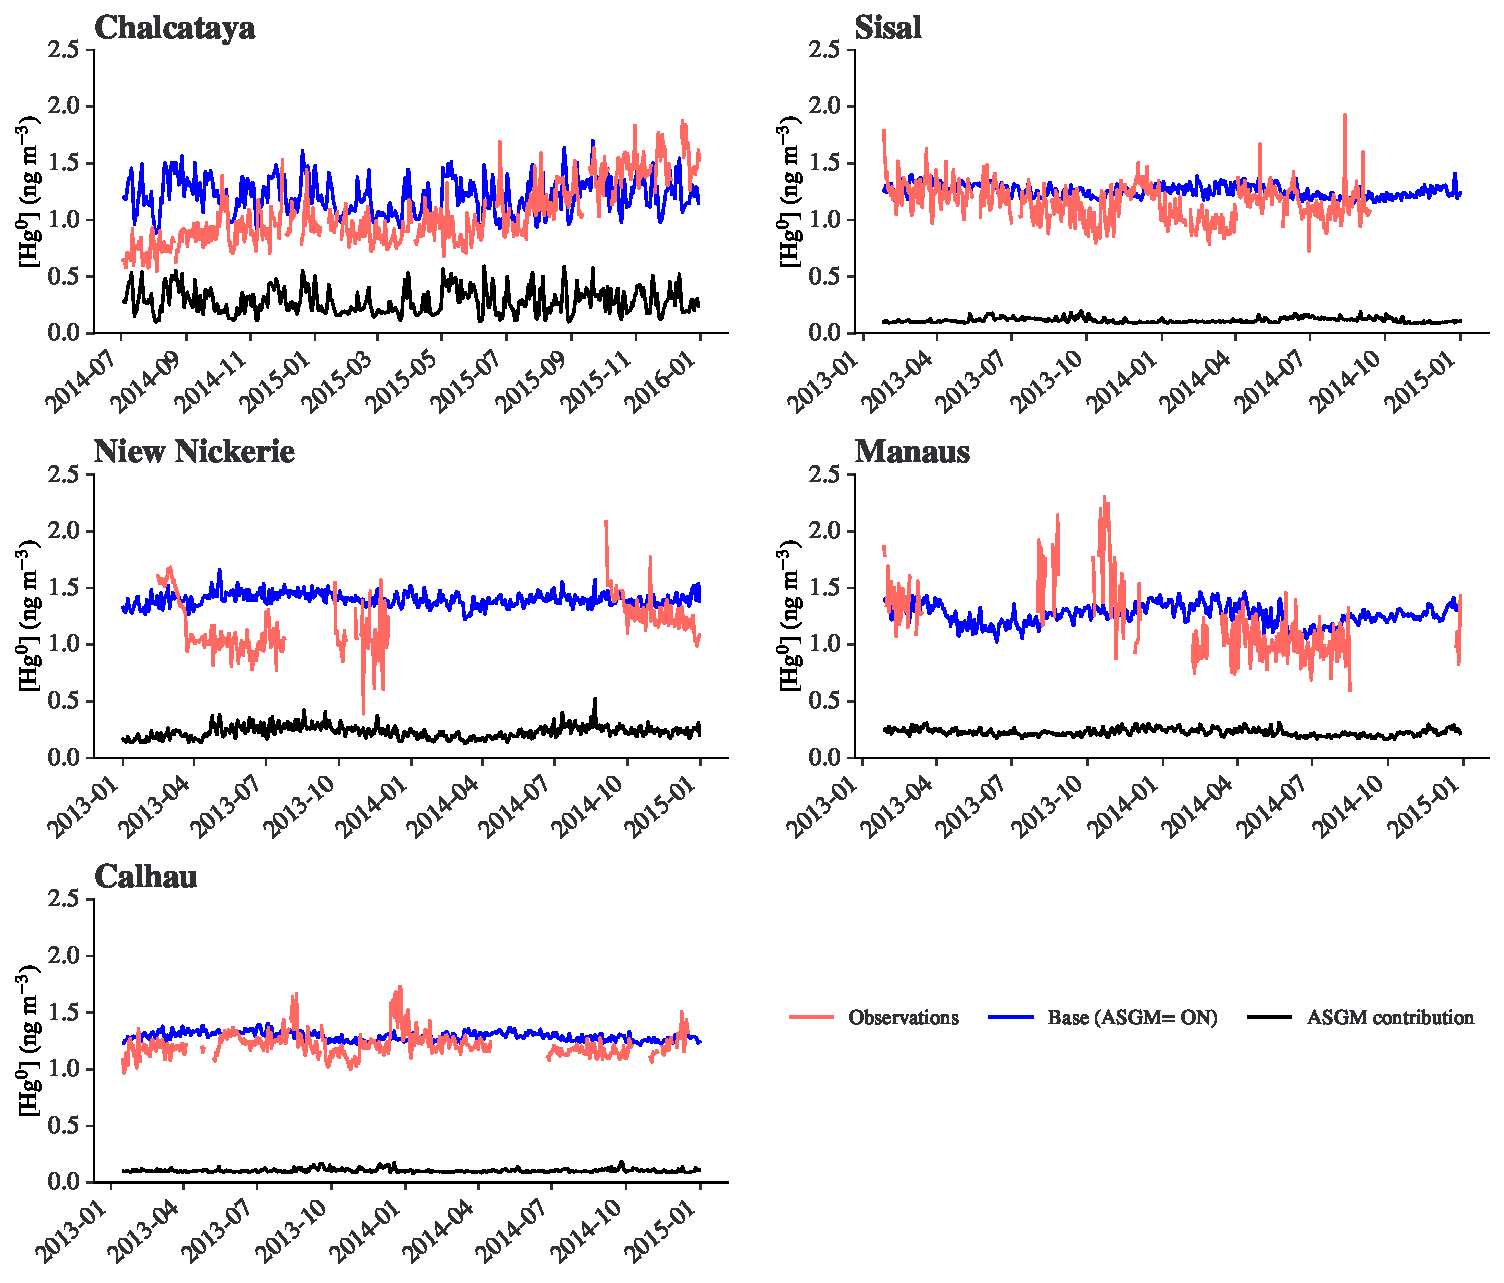
\includegraphics[width=\textwidth]{templates/figures/GMOS_Sites/GMOS_Sites.pdf}
\centering
\captionof{figure}{Time series plots of the observed TGM concentrations at different GMOS sites in red with the corresponding modeled concentration in blue and the associated ASGM contribution in green. Except for the CHC site, where the data are from July 2014 and January 2016, the available data and corresponding model outputs were plotted between January 2013 and January 2016.}
\label{fig:GMOSvsGC}
\end{figure}
\FloatBarrier


\begin{flushleft}


 This study also compared observed and modeled data on a daily resolution as seen in Figure \ref{fig:GMOSvsGC}, which shows the time series of the modeled \hgc in the atmosphere alongside the observed Hg and the simulated ASGM contribution to the atmospheric Hg concentration at the GMOS sites. The \gc model version used in this study overestimated the concentration of Hg on most days. However, the \gc estimated average \hgc over the available observation period was within one standard deviation of the observed Hg in most of the sites except for the Manaus and Nieuw Nickerie sites. \gcs overestimates the observed GEM concentrations at the Manaus and Bariloche master sites by over 25\%  and the GEM concentration at Nieuw Nickerie by 20\%, which may be indicative of poor parameterization of GEM in the model. In particular, the overestimation of the GEM concentration at Manaus further indicates the model's poor parameterization of Hg vegetation uptake.
\end{flushleft}


\begin{figure}[H]
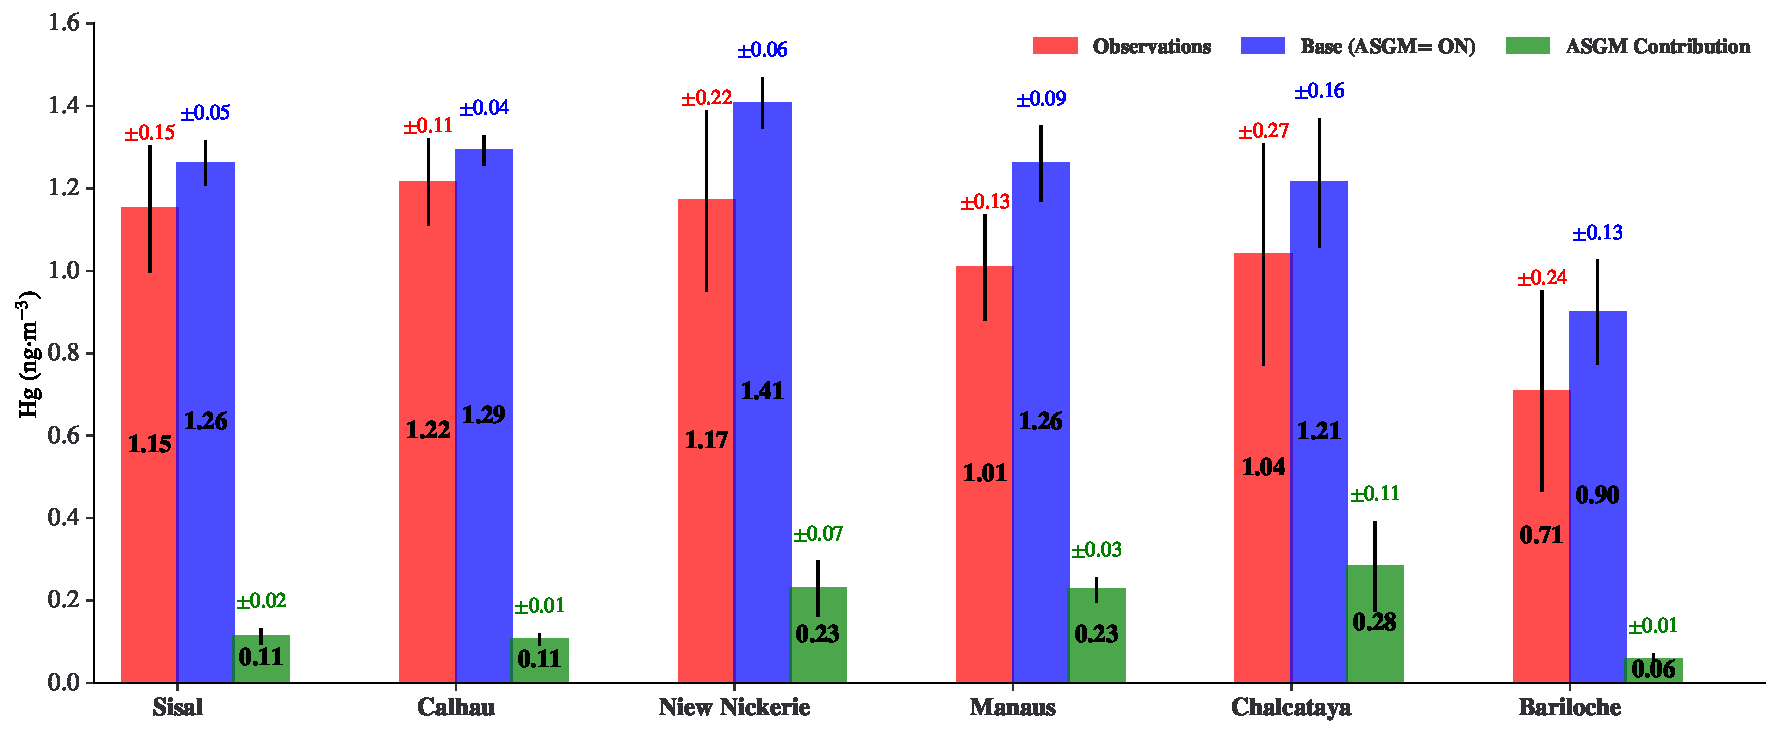
\includegraphics[width=\textwidth]{templates/figures/GMOS_Sites/gmos_sites_stats.pdf}
\centering
\captionof{figure}{Bar chart comparing the modeled average Hg concentration  at the respective GMOS Sites}
\label{fig:gmos_sites_stats}
\end{figure}
\FloatBarrier
\begin{flushleft}
Moreover, Figure \ref{fig:GMOSvsGC} and Figure \ref{fig:gmos_sites_stats} clearly show that ASGMs modeled contribution is low in most of the sites except for Calcataya, Manaus, and Nieuw Nickerie. This behavior of the model regarding the predicted ASGM contribution at these sites is not surprising since these three sites are in countries estimated to be among the top 10 Latin American ASGM Hg emitters. 
\end{flushleft}

\begin{table}[H]
\captionof{table}{Table showing the extent to which the model predicts the observations showed by the percentage difference between the model predictions and the observations }
\label{tab:model_percentage_overestimation_of_mean}

\center
\resizebox{0.7\textwidth}{!}{\begin{tabular}{lccc}
  \hline

GMOS Site       & Observed Average          & Modeled Average   &Percentage difference between \\
                & TGM/GEM Concentration     & \hg Concentration      &modeled and observed mean (\%)  \\
                        
\hline
Sisal          &    1.15                &             1.26                      & 10     \\
Calhau         &     1.22               &               1.29                    & 6      \\
Nieuw Nickerie &     1.17               &               1.41                    & 20    \\
Manaus         &     1.01               &               1.26                    & 25     \\
Chalcataya     &     1.04               &               1.21                    & 17     \\
Bariloche      &     0.71               &               0.9                    & 27     \\
  \hline
\end{tabular}}

\end{table}


\begin{flushleft}
  \begin{figure}[H]
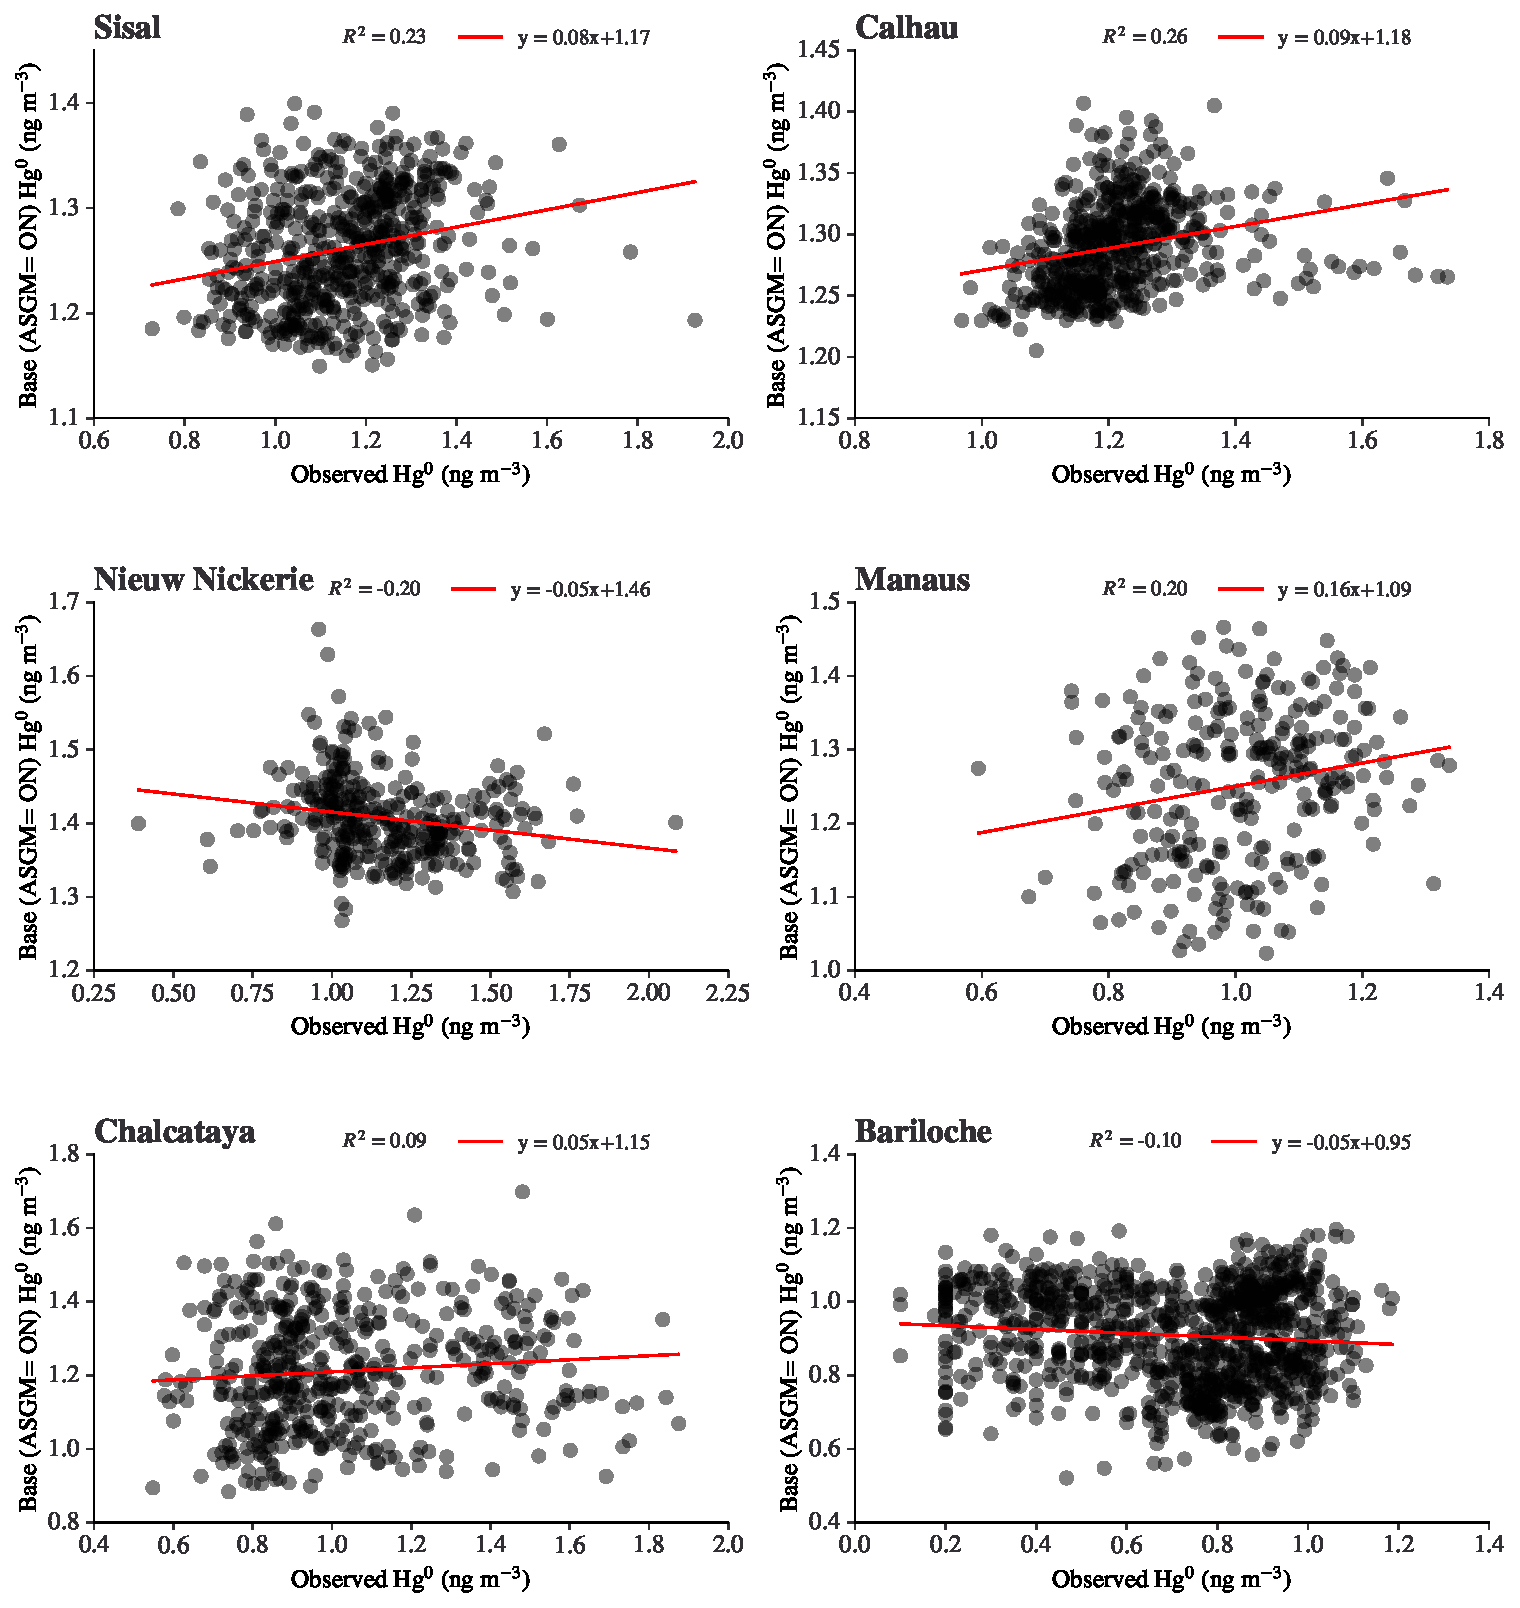
\includegraphics[width=0.8\textwidth]{templates/figures/GMOS_Sites/gmos_sites_scatter.pdf}
\centering
\captionof{figure}{Time series plots of the observed TGM concentrations at different GMOS sites in red with the corresponding modeled concentration in blue and the associated ASGM contribution in black. Available observations and corresponding model output between January 2013 and January 2015 were plotted except for the CHC site, whose data is from July 2014 and January 2016}
\label{fig:gmos_sites_scatter}
\end{figure}
\FloatBarrier
\end{flushleft}

\begin{flushleft}
A striking trend in most plots of the observed vs modeled Hg concentration in Figure \ref{fig:gmos_sites_scatter} is the GEOS-Chem model's general overestimation of the Hg concentration and mismatch in the variability. The observed average daily TGM concentration at the GMOS sites (red line) is compared to the modeled \on average daily \hg (blue line) and the ASGM contribution (black line). The different Hg concentrations were plotted as a function of time-based on the availability of data records between 2012 and 2016. None of the sites had a continuous data set that spanned the entire period of interest, but the Niew Nickerie and Manaus sites had the most minor data records at 215 days and 100 days, respectively, as seen in Table \ref{tab:ASGM_at_GMOS_annual_avs}.   
\end{flushleft}

\begin{flushleft}
 
\end{flushleft}


\subsection{Passive Sampler Observations vs GEOS-Chem}


\begin{flushleft}


\end{flushleft}











\section{Conclusion}

